\chapter{REST APIs}\label{rest-apis}

\section{API Review}\label{api-review}

\begin{itemize}
\tightlist
\item
  An API (Application Programming Interface) is a software interface
  that allows two applications to communicate with each other.
\item
  APIs are essential not just for network automation but for all kinds
  of applications
\item
  In SDN Architecture, APIs are use to communicate between apps and the
  SDN controller (via the NBI) and between the SDN controller and the
  network devices (via the SBI)
\item
  The NBI typically uses REST APIs
\item
  NETCONF and RESTCONF are popular Southbound APIs
\end{itemize}

\section{CRUD Operations and HTTP
Verbs}\label{crud-operations-and-http-verbs}

\begin{itemize}
\item
  CRUD ( CREATE, READ, UPDATE, DELETE) refers to the operations we
  perform using REST APIs
\item
  CREATE :

  \begin{itemize}
  \tightlist
  \item
    Used to CREATE new variables and set their initial values

    \begin{itemize}
    \tightlist
    \item
      Example: create a variable ``ip\_address'' and set the value to
      ``10.1.1.1''
    \end{itemize}
  \end{itemize}
\item
  READ :

  \begin{itemize}
  \tightlist
  \item
    Used to READ the value of a variable

    \begin{itemize}
    \tightlist
    \item
      Example: Read the value of variable ``ip\_address'' (''10.1.1.1'')
    \end{itemize}
  \end{itemize}
\item
  UPDATE :

  \begin{itemize}
  \tightlist
  \item
    Used to CHANGE / UPDATE the value of a variable

    \begin{itemize}
    \tightlist
    \item
      Example: Change the value of ``ip\_address'' from ``10.1.1.1'' to
      ``10.2.3.4''
    \end{itemize}
  \end{itemize}
\item
  DELETE :

  \begin{itemize}
  \tightlist
  \item
    Used to DELETE variables

    \begin{itemize}
    \tightlist
    \item
      Example: Delete variable ``ip\_address''
    \end{itemize}
  \end{itemize}
\item
  HTTP uses \emph{verbs} (aka. methods) that map to these CRUD
  operations
\item
  REST APIs typically use HTTP
\end{itemize}

\begin{figure}
\centering
\pandocbounded{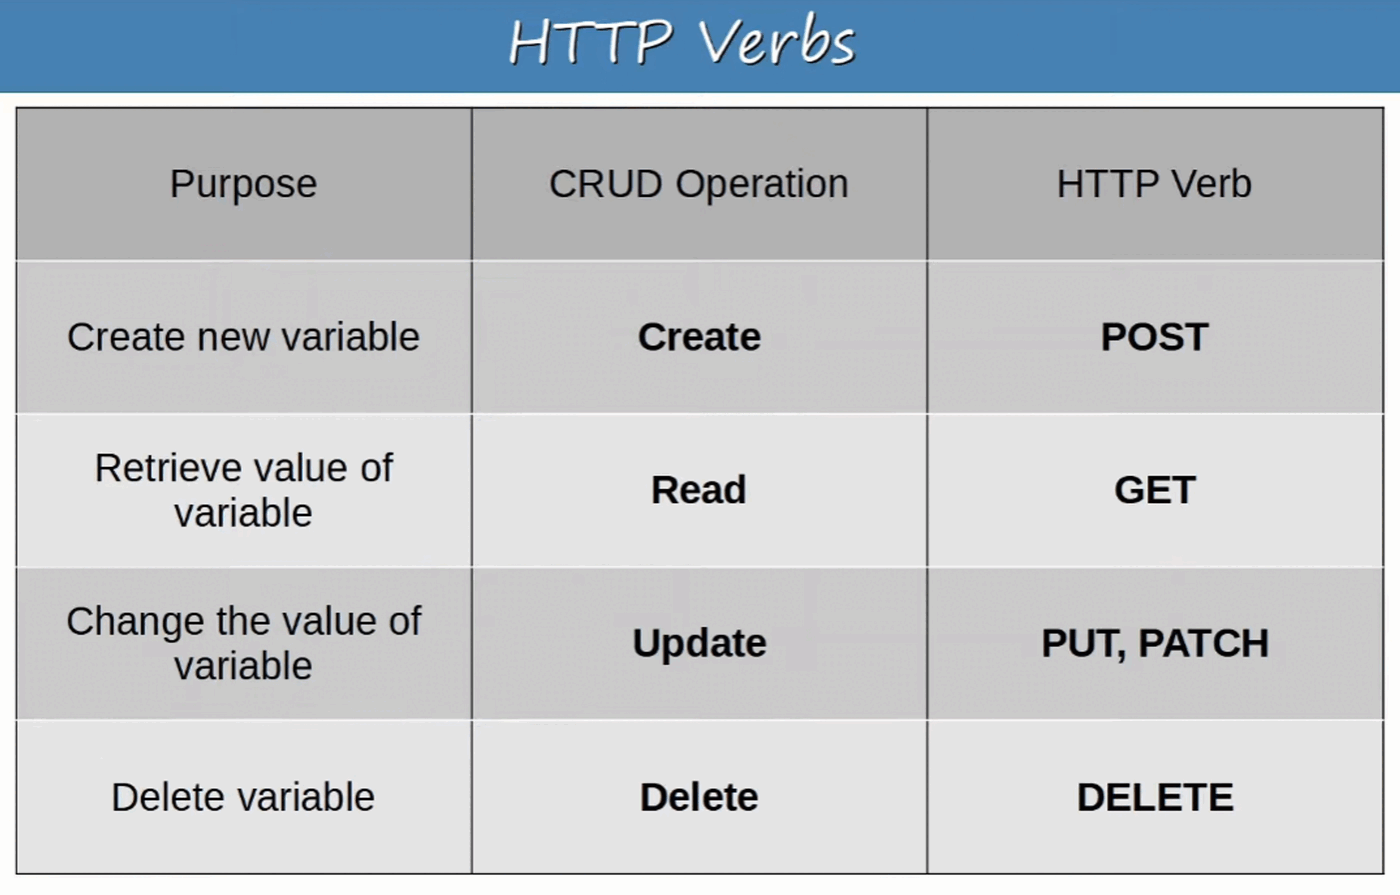
\includegraphics[keepaspectratio,alt={image}]{images/64-rest-apis/img-001.png}}
\end{figure}

\section{HTTP Request}\label{http-request}

\begin{itemize}
\tightlist
\item
  When an HTTP client sends a request to an HTTP server, the HTTP header
  includes information like this:

  \begin{itemize}
  \tightlist
  \item
    An HTTP Verb (ie: GET)
  \item
    A URI (Uniform Resource Identifier) indicating the resource it is
    trying to access
  \end{itemize}
\end{itemize}

\begin{figure}
\centering
\pandocbounded{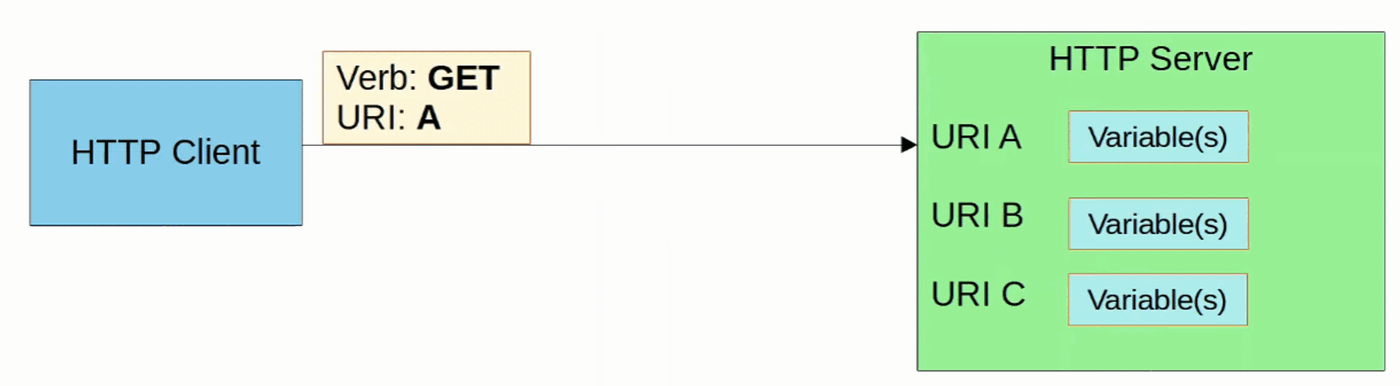
\includegraphics[keepaspectratio,alt={image}]{images/64-rest-apis/img-002.png}}
\end{figure}

An example of a URI (demonstrated later)

\begin{figure}
\centering
\pandocbounded{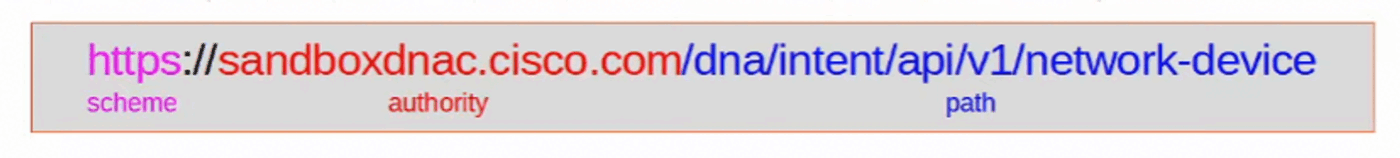
\includegraphics[keepaspectratio,alt={image}]{images/64-rest-apis/img-003.png}}
\end{figure}

\begin{itemize}
\tightlist
\item
  The HTTP request can include additional headers which pass additional
  information to the server.
\end{itemize}

Check the list at
\url{https://developer.mozilla.org/en-US/docs/Web/HTTP/Headers}

\begin{figure}
\centering
\pandocbounded{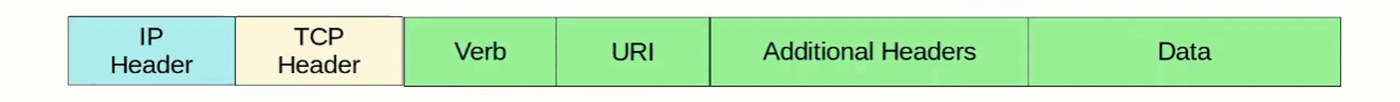
\includegraphics[keepaspectratio,alt={image}]{images/64-rest-apis/img-004.png}}
\end{figure}

\begin{itemize}
\item
  An example would be an ACCEPT header, which informs the server about
  the types(s) of data that can be sent back to the client.

  \begin{itemize}
  \tightlist
  \item
    Example: \textbf{Accept: application/json} or \textbf{Accept:
    application/xml}
  \end{itemize}
\item
  You can also view standard HTTP header fields with some examples at
  \url{https://en.wikipedia.org/wiki/List_of_HTTP_header_fields}
\item
  When a REST client makes an API call (request) to a REST server, it
  will send an HTTP request like the one above
\end{itemize}

\begin{quote}
REST APIs do NOT have to use HTTP for communication, although HTTP is
the most common choice
\end{quote}

\section{HTTP Response}\label{http-response}

\begin{itemize}
\tightlist
\item
  The server's response will include a STATUS CODE indicating if the
  request succeeded or failed, as well as other details
\item
  The FIRST digit indicates the class of the response:

  \begin{itemize}
  \tightlist
  \item
    1xx : Informational - request was received, continuing process
  \item
    2xx : Successful - request was successfully received, understood,
    and accepted
  \item
    3xx : Redirection - further action needs to be taken in order to
    complete the request
  \item
    4xx : Client Error - request contains bad syntax or cannot be
    fulfilled
  \item
    5xx : Server Error - server failed to fulfill an apparently valid
    request
  \end{itemize}
\end{itemize}

\begin{figure}
\centering
\pandocbounded{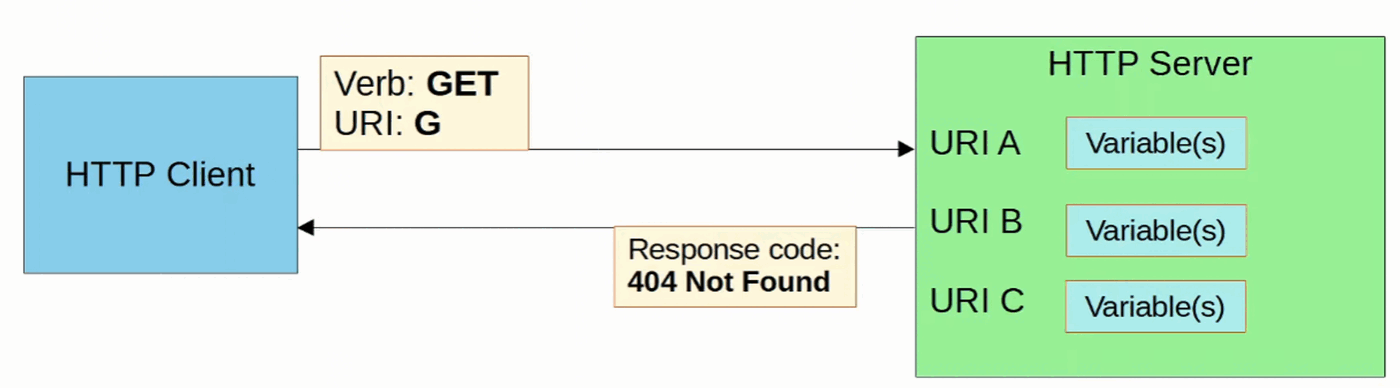
\includegraphics[keepaspectratio,alt={image}]{images/64-rest-apis/img-005.png}}
\end{figure}

Examples of each HTTP Response class:

\begin{itemize}
\tightlist
\item
  1xx Informational

  \begin{itemize}
  \tightlist
  \item
    102 Processing indicates that the server received the request and is
    processing it but the response is not available yet
  \end{itemize}
\item
  2xx Successful

  \begin{itemize}
  \tightlist
  \item
    200 OK **indicates that the request succeeded
  \item
    201 Created indicates the request succeeded and a new resource was
    created
  \end{itemize}
\item
  3xx Redirection

  \begin{itemize}
  \tightlist
  \item
    301 Moved Permanently indicates that the request resource has been
    moved and the server indicates its new location
  \end{itemize}
\item
  4xx Client Error

  \begin{itemize}
  \tightlist
  \item
    403 Unauthorized means the client must authenticate to get a
    response
  \item
    404 Not Found means the requested resource was not found
  \end{itemize}
\item
  5xx Server Error

  \begin{itemize}
  \tightlist
  \item
    500 Internal Server Error means the server encountered something
    unexpected that it doesn't know how to handle
  \end{itemize}
\end{itemize}

REST APIs

\begin{itemize}
\tightlist
\item
  REST stands for Representational State Transfer
\item
  REST APIs are also know as REST-based APIs or RESTful APIs

  \begin{itemize}
  \tightlist
  \item
    REST isn't a specific API. Instead it describes a set of rules about
    how the API should work
  \end{itemize}
\item
  The SIX constraints of RESTful architecture are:

  \begin{itemize}
  \tightlist
  \item
    Stateless
  \item
    Layered system
  \item
    Uniform Interface
  \item
    Client-Server
  \item
    Cacheable or non-cacheable
  \item
    Code-on-Demand (optional)
  \end{itemize}
\item
  For applications to communicate over a network, networking protocols
  must be used to facilitate those communications

  \begin{itemize}
  \tightlist
  \item
    For REST APIs, HTTP(S) is the most common choice
  \end{itemize}
\end{itemize}

REST: Client-Server

\begin{itemize}
\tightlist
\item
  REST APIs use a client-server architecture
\item
  The client uses API calls (HTTP requests) to access the resources on
  the server
\item
  The separation between the client and server means they can both
  change and evolve independently of each other

  \begin{itemize}
  \tightlist
  \item
    When the client application changes or the server application
    changes, the interface between them must not break
  \end{itemize}
\end{itemize}

\begin{figure}
\centering
\pandocbounded{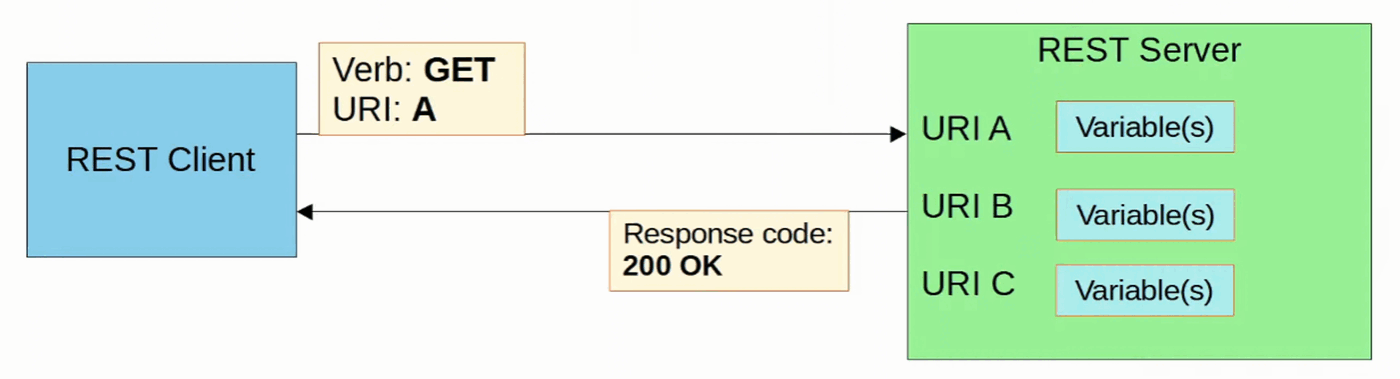
\includegraphics[keepaspectratio,alt={image}]{images/64-rest-apis/img-006.png}}
\end{figure}

REST: Stateless

\begin{itemize}
\tightlist
\item
  REST APIs exchanges are STATELESS
\item
  This means that each API exchange is a separate event, independent of
  all past exchanges between the client and server

  \begin{itemize}
  \tightlist
  \item
    The server does not store information about previous requests from
    the client to determine how it should respond to new requests
  \end{itemize}
\item
  If authentication is required, this means that the client must
  authenticate with the server for each request it makes
\item
  TCP is an example of a STATEFUL protocol
\item
  UDP is an example of STATELESS protocol
\end{itemize}

** Although REST APIs use HTTP, which uses TCP (STATEFUL) as it's LAYER
4 protocol, HTTP and REST APIs themselves aren't STATEFUL. The functions
of each layer are separate !

REST: Cacheable or Non-Cacheable

\begin{itemize}
\tightlist
\item
  REST APIs must support caching of data
\item
  \emph{Caching} refers to storing data for future use

  \begin{itemize}
  \tightlist
  \item
    Example :

    \begin{itemize}
    \tightlist
    \item
      Your computer might cache many elements of a web page so it
      doesn't have to retrieve the entire page every time you visit.
      This improves performance for the client and reduces load on the
      server
    \end{itemize}
  \end{itemize}
\item
  Not all resources have to be cacheable but cacheable resources MUST be
  declared as cacheable
\end{itemize}

\section{For the CCNA}\label{for-the-ccna}

\begin{figure}
\centering
\pandocbounded{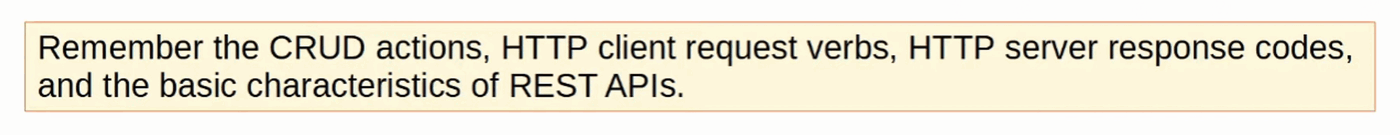
\includegraphics[keepaspectratio,alt={image}]{images/64-rest-apis/img-007.png}}
\end{figure}

\section{REST API Calls Using Cisco
DEVNET}\label{rest-api-calls-using-cisco-devnet}

\begin{itemize}
\item
  ``Cisco DevNet is Cisco's developer program to help developers and IT
  professionals who want to write applications and develop integrations
  with Cisco products, platforms, and API's''
\item
  DevNet offers lots of free resources such as courses, tutorials, labs,
  sandboxes, documentation, etc to learn about AUTOMATION and develop
  your skills
\item
  There is also a DevNet certification track that you can pursue if you
  are interested in AUTOMATION
\item
  We will use their Cisco DNA Center Sandbox to send a REST API call
  using Postman

  \begin{itemize}
  \tightlist
  \item
    DNA Center is one of Cisco's SDN Controllers (covered in more detail
    later)
  \item
    Postman is a platform for building an using APIs
  \end{itemize}
\end{itemize}

\section{To Start}\label{to-start}

\begin{itemize}
\tightlist
\item
  Make an account on
  \href{http://developer.cisco.com}{developer.cisco.com} (Used my
  NetAcademy login)
\item
  Make an accounts on \href{http://postman.com}{postman.com} and
  download the desktop app (\url{https://www.postman.com/downloads}) -
  Used my \href{http://gmail.com}{gmail.com} account
\end{itemize}
